\documentclass[aspectratio=169,11pt]{beamer}
\usetheme{Madrid}
\usecolortheme{default}
\usepackage{fontspec}
\usepackage{unicode-math}
\usepackage{tikz}
\usetikzlibrary{arrows.meta,positioning,shapes.geometric,calc,fit,backgrounds}
\usepackage{booktabs}
\usepackage{xcolor}
\usepackage{hyperref}
\usepackage{listings}

\setsansfont{DejaVu Sans}
\setmonofont{DejaVu Sans Mono}

\definecolor{factoryBlue}{HTML}{2E6BE6}
\definecolor{factoryInk}{HTML}{1C2331}
\definecolor{factorySlate}{HTML}{596579}
\definecolor{factoryMint}{HTML}{1EAD8F}
\definecolor{factoryAmber}{HTML}{F5A623}
\definecolor{factoryRed}{HTML}{E35D6A}
\definecolor{factoryBg}{HTML}{F6F8FC}
\definecolor{factoryPanel}{HTML}{FFFFFF}
\definecolor{factoryLine}{HTML}{D9E1F2}

\setbeamercolor{normal text}{fg=factoryInk,bg=factoryBg}
\setbeamercolor{frametitle}{fg=factoryInk,bg=factoryBg}
\setbeamercolor{title}{fg=factoryInk}
\setbeamercolor{subtitle}{fg=factorySlate}
\setbeamercolor{structure}{fg=factoryBlue}
\setbeamercolor{block title}{fg=white,bg=factoryBlue}
\setbeamercolor{block body}{fg=factoryInk,bg=white}
\setbeamertemplate{navigation symbols}{}
\setbeamertemplate{footline}{%
  \leavevmode\hbox{\begin{beamercolorbox}[wd=.72\paperwidth,ht=2.6ex,dp=1ex,leftskip=2em]{author in head/foot}\scriptsize Factory - development process knowledge base\end{beamercolorbox}%
  \begin{beamercolorbox}[wd=.28\paperwidth,ht=2.6ex,dp=1ex,rightskip=2em plus1fil]{date in head/foot}\scriptsize \insertframenumber/\inserttotalframenumber\end{beamercolorbox}}}

\newcommand{\pill}[2]{\tikz[baseline=(X.base)]\node[fill=#1!12,draw=#1!45,rounded corners=8pt,inner xsep=8pt,inner ysep=3pt,text=#1,font=\scriptsize\bfseries](X){#2};}
\newcommand{\bigmetric}[2]{\begin{minipage}{0.23\linewidth}\centering{\Large\bfseries #1}\\[-1mm]{\scriptsize\color{factorySlate}#2}\end{minipage}}
\newcommand{\card}[2]{\begin{block}{#1}\small #2\end{block}}

\title{Factory}
\subtitle{Documenting, explaining, and spreading our development process}
\author{Engineering practice initiative}
\date{2026-05-19}

\begin{document}

{\setbeamertemplate{footline}{}\begin{frame}[plain]
\begin{columns}[onlytextwidth]
\column{.23\paperwidth}
\begin{tikzpicture}
  \fill[factoryBlue] (0,0) rectangle (3.15,7.2);
  \foreach \y in {.9,1.8,...,6.3}{\draw[white,opacity=.18,line width=.8pt] (.3,\y) -- (2.9,\y+.35);}  
\end{tikzpicture}
\column{.72\paperwidth}
\vspace{8mm}
{\fontsize{42}{46}\selectfont\bfseries Factory}\par
\vspace{4mm}
{\fontsize{26}{31}\selectfont\bfseries Development as a reproducible process}\par
\vspace{6mm}
{\large\color{factorySlate} How we turn messy problems into shipped, verified, documented improvements - without losing context.}\par
\vspace{9mm}
\pill{factoryMint}{epics}\hspace{2mm}\pill{factoryBlue}{review loops}\hspace{2mm}\pill{factoryAmber}{verification gates}\hspace{2mm}\pill{factoryRed}{observability}
\vfill
{\color{factorySlate} Starter deck / 2026-05-19}
\end{columns}
\end{frame}}

\begin{frame}{Why Factory exists}
\large

For a long time, the bottleneck was speed.

\vspace{4mm}

We knew how to build software, but many useful feedback loops were too expensive to create, run, or maintain:
tests, reviews, diagnostics, gates, examples, documentation, migrations, and repeated verification.

\vspace{5mm}

Recent AI systems changed the economics.

\vspace{4mm}

Factory exists to capture that change:
not by freezing work into a framework,
but by making feedback loops cheap enough to build continuously.

\vspace{5mm}

\centering
\pill{factoryBlue}{The product is not the framework. The product is the loop.}

\end{frame}


\begin{frame}{What Factory means by reproducible}
\large
Factory does not claim that every software outcome is bit-for-bit reproducible.

\vspace{5mm}

It aims to make the \textbf{development process} reproducible:

\vspace{3mm}

\begin{itemize}
\item how we frame ambiguous problems;
\item how we slice work into epics;
\item how we preserve context and decisions;
\item how we verify changes;
\item how we capture reviewer feedback;
\item how we turn incidents and fixes into reusable knowledge.
\end{itemize}

\vspace{4mm}

\centering
\pill{factoryBlue}{Reproducible process, bounded system, evidence-driven confidence}
\end{frame}

\begin{frame}{The process in one sentence}
\begin{center}
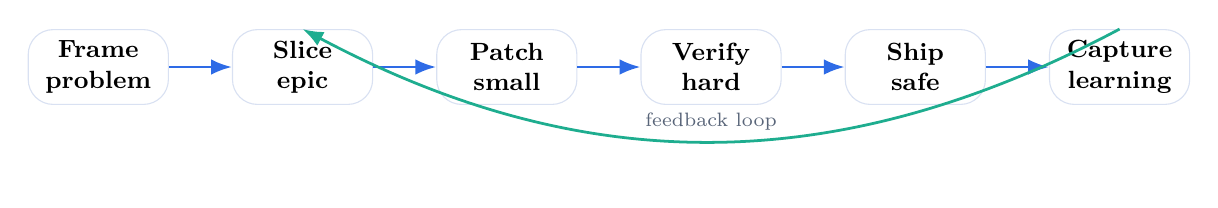
\begin{tikzpicture}[node distance=.8cm,>=Latex]
  \tikzstyle{stepbox}=[draw=factoryLine,fill=white,rounded corners=9pt,minimum width=1.78cm,minimum height=.95cm,align=center,font=\small\bfseries]
  \node[stepbox] (problem) {Frame\\problem};
  \node[stepbox,right=of problem] (slice) {Slice\\epic};
  \node[stepbox,right=of slice] (patch) {Patch\\small};
  \node[stepbox,right=of patch] (verify) {Verify\\hard};
  \node[stepbox,right=of verify] (ship) {Ship\\safe};
  \node[stepbox,right=of ship] (learn) {Capture\\learning};
  \foreach \a/\b in {problem/slice,slice/patch,patch/verify,verify/ship,ship/learn}{\draw[->,line width=1pt,draw=factoryBlue] (\a) -- (\b);}  
  \draw[->,line width=1pt,draw=factoryMint,bend left=28] (learn.north) to node[above,font=\scriptsize\color{factorySlate}]{feedback loop} (slice.north);
\end{tikzpicture}
\end{center}
\vspace{7mm}
\begin{columns}[T]
\column{.48\textwidth}
\textbf{Operating principle}\par\smallskip
\small Every change should leave behind enough evidence for a future engineer to understand what changed, why, how it was verified, and what remains risky.
\column{.48\textwidth}
\textbf{Anti-goal}\par\smallskip
\small Do not turn development into ceremony. Factory documents the shortest reliable path from ambiguity to confidence.
\end{columns}
\end{frame}

\begin{frame}{Factory converts tacit work into explicit assets}
\begin{columns}[T]
\column{.52\textwidth}
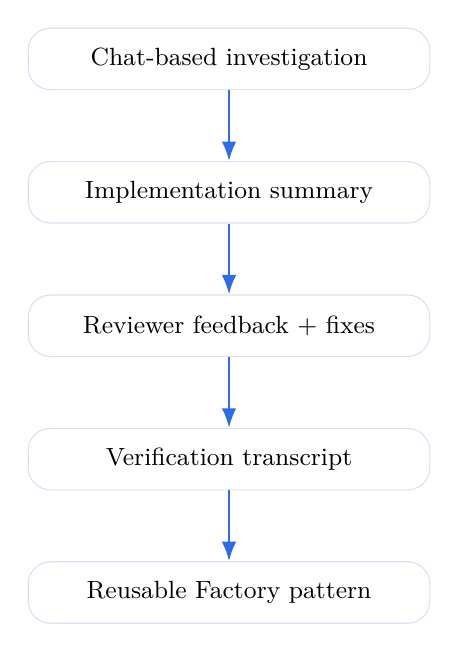
\begin{tikzpicture}[>=Latex, node distance=9mm]
\tikzstyle{box}=[draw=factoryLine,fill=white,rounded corners=8pt,minimum width=5.1cm,minimum height=.78cm,align=left,font=\small]
\node[box] (a) {Chat-based investigation};
\node[box,below=of a] (b) {Implementation summary};
\node[box,below=of b] (c) {Reviewer feedback + fixes};
\node[box,below=of c] (d) {Verification transcript};
\node[box,below=of d] (e) {Reusable Factory pattern};
\foreach \x/\y in {a/b,b/c,c/d,d/e}{\draw[->,draw=factoryBlue,line width=.9pt] (\x) -- (\y);}  
\end{tikzpicture}
\column{.44\textwidth}
\textbf{Outputs we want}\par\medskip
\small
\begin{itemize}
\item Playbooks for recurring work
\item Checklists for risky changes
\item Example PRs with narrative
\item CI/gate design notes
\item Debugging recipes
\item Onboarding modules
\end{itemize}
\end{columns}
\end{frame}

\begin{frame}{A Factory epic has a standard shape}
\begin{center}
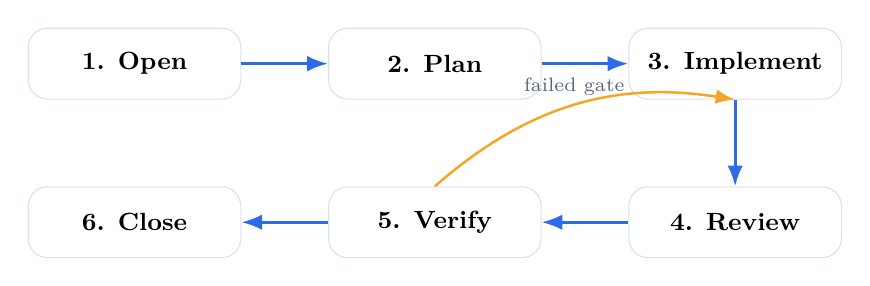
\begin{tikzpicture}[node distance=1.1cm,>=Latex]
\tikzstyle{stage}=[draw=factoryLine,fill=white,rounded corners=7pt,minimum width=2.7cm,minimum height=.9cm,align=center,font=\small\bfseries]
\node[stage] (open) {1. Open};
\node[stage,right=of open] (plan) {2. Plan};
\node[stage,right=of plan] (implement) {3. Implement};
\node[stage,below=of implement] (review) {4. Review};
\node[stage,left=of review] (verify) {5. Verify};
\node[stage,left=of verify] (close) {6. Close};
\foreach \a/\b in {open/plan,plan/implement,implement/review,review/verify,verify/close}{\draw[->,draw=factoryBlue,line width=1pt] (\a) -- (\b);}  
\draw[->,draw=factoryAmber,line width=.9pt,bend left=25] (verify.north) to node[above,font=\scriptsize\color{factorySlate}]{failed gate} (implement.south);
\end{tikzpicture}
\end{center}
\vspace{4mm}
\small
\begin{tabular}{@{}p{.2\linewidth}p{.72\linewidth}@{}}
\toprule
\textbf{Part} & \textbf{What gets captured} \\
\midrule
Problem & Symptom, operator impact, current evidence, constraints. \\
Plan & Small slices, risk boundaries, verification strategy. \\
Closeout & Files changed, tests run, unresolved follow-ups, rollout notes. \\
\bottomrule
\end{tabular}
\end{frame}

\begin{frame}{Verification is part of the product, not a cleanup step}
\begin{columns}[T]
\column{.46\textwidth}
\textbf{Factory asks for evidence at each layer}\par\medskip
\small
\begin{itemize}
\item Static checks: format, lint, type checks
\item Unit and widget tests
\item Integration and fixture regressions
\item Artifact sanity checks
\item Deployment gates and post-deploy observation
\end{itemize}
\column{.5\textwidth}
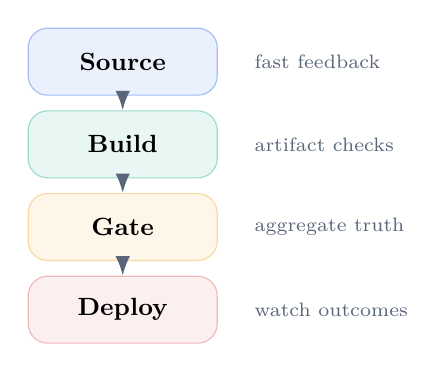
\begin{tikzpicture}[>=Latex]
\foreach \i/\name/\col in {0/Source/factoryBlue,1/Build/factoryMint,2/Gate/factoryAmber,3/Deploy/factoryRed}{
  \node[draw=\col!45,fill=\col!10,rounded corners=7pt,minimum width=2.4cm,minimum height=.85cm,font=\small\bfseries] (n\i) at (0,-\i*1.05) {\name};
}
\foreach \i in {0,1,2}{\pgfmathtruncatemacro{\j}{\i+1}\draw[->,draw=factorySlate,line width=.9pt] (n\i) -- (n\j);}
\node[anchor=west,align=left,font=\scriptsize\color{factorySlate}] at (1.55,0) {fast feedback};
\node[anchor=west,align=left,font=\scriptsize\color{factorySlate}] at (1.55,-1.05) {artifact checks};
\node[anchor=west,align=left,font=\scriptsize\color{factorySlate}] at (1.55,-2.1) {aggregate truth};
\node[anchor=west,align=left,font=\scriptsize\color{factorySlate}] at (1.55,-3.15) {watch outcomes};
\end{tikzpicture}
\end{columns}
\vspace{3mm}
\centering\pill{factoryBlue}{Rule of thumb: if a reviewer can ask “how do we know?”, the Factory artifact should already answer.}
\end{frame}

\begin{frame}{Review loops are structured, not adversarial}
\begin{columns}[T]
\column{.49\textwidth}
\card{Reviewer role}{Find hidden risk, force precision, and turn vague confidence into explicit evidence.}
\card{Implementer role}{Respond with scoped patches, verification, and concise summaries.}
\column{.49\textwidth}
\card{Factory role}{Preserve the pattern: what kind of issue was caught, how it was fixed, and how it becomes a future checklist item.}
\card{Outcome}{Every review improves both the code and the development system.}
\end{columns}
\end{frame}

\begin{frame}{Instrumentation-first debugging}
\large
When a system behaves strangely, Factory prefers visibility over guessing.
\vspace{5mm}
\begin{center}
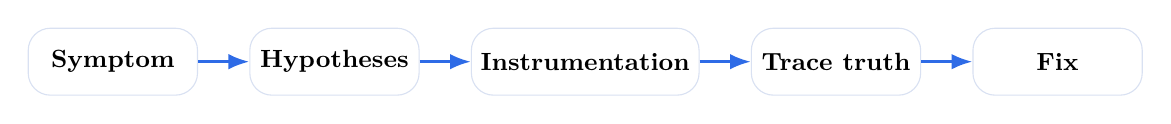
\begin{tikzpicture}[>=Latex,node distance=.65cm]
\tikzstyle{nodebox}=[draw=factoryLine,fill=white,rounded corners=8pt,minimum width=2.15cm,minimum height=.85cm,align=center,font=\small\bfseries]
\node[nodebox] (symptom) {Symptom};
\node[nodebox,right=of symptom] (hyp) {Hypotheses};
\node[nodebox,right=of hyp] (instr) {Instrumentation};
\node[nodebox,right=of instr] (truth) {Trace truth};
\node[nodebox,right=of truth] (fix) {Fix};
\foreach \a/\b in {symptom/hyp,hyp/instr,instr/truth,truth/fix}{\draw[->,draw=factoryBlue,line width=1pt] (\a) -- (\b);}  
\end{tikzpicture}
\end{center}
\vspace{5mm}
\small
Examples: timing breakdowns, trace diagnostics, synthetic/no-trace classifications, debug endpoints, stale artifact flags, deployment gate status files.
\end{frame}

\begin{frame}{Factory knowledge map}
\begin{center}
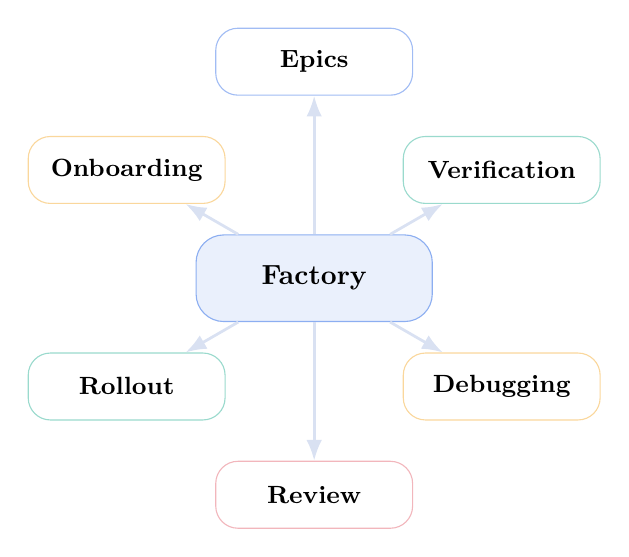
\begin{tikzpicture}[>=Latex]
\node[draw=factoryBlue!55,fill=factoryBlue!10,rounded corners=10pt,minimum width=3.0cm,minimum height=1.1cm,font=\bfseries] (center) {Factory};
\foreach \angle/\name/\col in {90/Epics/factoryBlue,30/Verification/factoryMint,-30/Debugging/factoryAmber,-90/Review/factoryRed,-150/Rollout/factoryMint,150/Onboarding/factoryAmber}{
  \node[draw=\col!45,fill=white,rounded corners=8pt,minimum width=2.5cm,minimum height=.85cm,font=\small\bfseries] (x\angle) at (\angle:2.75cm) {\name};
  \draw[->,draw=factoryLine,line width=1pt] (center) -- (x\angle);
}
\end{tikzpicture}
\end{center}
\end{frame}

\begin{frame}{First content tracks}
\small
\begin{tabular}{@{}p{.25\linewidth}p{.42\linewidth}p{.24\linewidth}@{}}
\toprule
\textbf{Track} & \textbf{Starter artifact} & \textbf{Audience} \\
\midrule
Epic lifecycle & How to run an implementation epic from symptom to closeout & Engineers, tech leads \\
Verification gates & Artifact-driven CI gates and deployment safety & Platform, DevOps, reviewers \\
Debugging playbooks & Instrumentation-first trace/debug method & Backend, SRE, support \\
Review patterns & Turning reviewer comments into reusable checks & Everyone shipping code \\
Rollout notes & How to ship risky changes with observability & Leads, operators \\
\bottomrule
\end{tabular}
\vspace{5mm}
\centering\pill{factoryBlue}{Start with real examples. Generalize only after the pattern has survived contact with production.}
\end{frame}

\begin{frame}{Suggested launch plan}
\begin{columns}[T]
\column{.33\textwidth}\card{1. Seed}{Create a short deck, a README, and 2-3 concrete case studies from recent work.}
\column{.33\textwidth}\card{2. Practice}{Use Factory language during active epics: plan, evidence, gate, closeout, follow-up.}
\column{.33\textwidth}\card{3. Spread}{Turn successful epics into brown bags, onboarding docs, and reusable templates.}
\end{columns}
\vspace{6mm}
\begin{center}
\bigmetric{1}{shared vocabulary}\hfill\bigmetric{3}{starter tracks}\hfill\bigmetric{30 min}{first internal talk}\hfill\bigmetric{ongoing}{living playbook}
\end{center}
\end{frame}

\begin{frame}{What good looks like}
\begin{center}
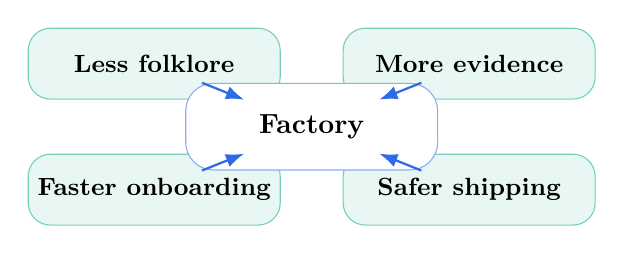
\begin{tikzpicture}[>=Latex]
\tikzstyle{good}=[draw=factoryMint!60,fill=factoryMint!10,rounded corners=8pt,minimum width=3.2cm,minimum height=.9cm,align=center,font=\small\bfseries]
\node[good] (a) at (0,1.6) {Less folklore};
\node[good] (b) at (4.0,1.6) {More evidence};
\node[good] (c) at (0,0) {Faster onboarding};
\node[good] (d) at (4.0,0) {Safer shipping};
\node[draw=factoryBlue!55,fill=white,rounded corners=10pt,minimum width=3.2cm,minimum height=1.1cm,font=\bfseries] (factory) at (2,0.8) {Factory};
\foreach \x in {a,b,c,d}{\draw[->,draw=factoryBlue,line width=.8pt] (factory) -- (\x);}  
\end{tikzpicture}
\end{center}
\vspace{4mm}
\large\centering
The end state is not “more documentation”.\par
It is a development process that teaches itself.
\end{frame}

\begin{frame}{FAQ: Factory Asked Questions}
\large

\begin{columns}[T]
\column{.33\textwidth}
\card{Can you sell me the Factory?}{
Sell what?

You can build your own. There is nothing to buy here.

Factory is a process, not a product.
}

\column{.33\textwidth}
\card{What do I need to build a Factory?}{
Feedback loops.

You need to build them, maintain them, and be part of them to some extent.
}

\column{.33\textwidth}
\card{What does my Factory need to evolve?}{
Time and energy.

The process improves only when real work keeps flowing through it.
}
\end{columns}

\vspace{5mm}
\centering
\pill{factoryBlue}{Factory is not installed. Factory is grown.}
\end{frame}

\begin{frame}[plain]
\begin{center}
\vspace{12mm}
{\fontsize{42}{46}\selectfont\bfseries Factory}\par\vspace{5mm}
{\Large Make the way we build more inspectable, repeatable, and reliable.}\par\vspace{10mm}
\pill{factoryBlue}{next: turn this deck into the Factory README and first playbook}
\end{center}
\end{frame}

\end{document}
